\documentclass[14pt, conference]{IEEEtran}
\ifCLASSINFOpdf
\else
\fi

\IEEEoverridecommandlockouts

\usepackage{listings}
\usepackage[table, svgnames]{xcolor}
\definecolor{codegreen}{rgb}{0,0.6,0}
\definecolor{codegray}{rgb}{0.5,0.5,0.5}
\definecolor{codepurple}{rgb}{0.58,0,0.82}
\definecolor{backcolour}{rgb}{0.5,1,0.5}
 
\lstdefinestyle{mystyle}{
    backgroundcolor=\color{backcolour},   
    commentstyle=\color{codegreen},
    keywordstyle=\color{magenta},
    numberstyle=\tiny\color{codegray},
    stringstyle=\color{codepurple},
    basicstyle=\footnotesize,
    breakatwhitespace=false,         
    breaklines=true,                 
    captionpos=b,                    
    keepspaces=true,                 
    numbers=none,                    
    numbersep=5pt,                  
    showspaces=false,                
    showstringspaces=false,
    showtabs=false,                  
    tabsize=2
}
 
\lstset{style=mystyle}


\usepackage{float}
\usepackage{longtable}
\usepackage{graphicx}
\usepackage{multirow}
%\usepackage{subcaption}
\usepackage{flushend}
\usepackage{hyperref}
\usepackage{tabularx} 
\usepackage{booktabs} % For formal tables
\usepackage{hhline}
\usepackage{array}

\colorlet{headercolour}{DarkSeaGreen}
\AtBeginEnvironment{tabular}{\rowcolors{1}{\ifnumequal{\rownum}{1}{headercolour}{white}}{}}%

\newcolumntype{L}[1]{>{\raggedright\let\newline\\\arraybackslash\hspace{0pt}}m{#1}}
\newcolumntype{C}[1]{>{\centering\let\newline\\\arraybackslash\hspace{0pt}}m{#1}}
\newcolumntype{R}[1]{>{\raggedleft\let\newline\\\arraybackslash\hspace{0pt}}m{#1}}
\bibliographystyle{IEEEtran}

\usepackage{cite}
\usepackage{amsmath,amssymb,amsfonts}
\usepackage{algorithmic}
\usepackage{graphicx}
\usepackage{textcomp}
\def\BibTeX{{\rm B\kern-.05em{\sc i\kern-.025em b}\kern-.08em
    T\kern-.1667em\lower.7ex\hbox{E}\kern-.125emX}}

\begin{document}

\title{Anomaly Detection Using Ensemble of Machine Learning Models}

\author{
\IEEEauthorblockN{Md. Khairul Islam\textsuperscript{1},
Prithula Hridi\textsuperscript{1}, Md. Shohrab Hossain\textsuperscript{1}, Husnu S. Narman\textsuperscript{2}}

\IEEEauthorblockA{\textsuperscript{1}Department of Computer Science and Engineering, Bangladesh University of Engineering and Technology, Bangladesh\\
    \textsuperscript{2}Weisberg Division of Computer Science, Marshall University, Huntington, WV, USA\\}
\IEEEauthorblockA{Email:  khairulislamtanim@gmail.com, prithula5117@gmail.com, mshohrabhossain@cse.buet.ac.bd,  narman@marshall.edu}
}

\maketitle

\begin{abstract}
Anomaly detection system plays a significant role in recognizing intruders or suspicious activities inside the system, catching unseen and unknown attacks. Despite it has the weakness of having high false alarm rate, it can detect zero day attacks effectively. However benchmark anomaly detection datasets on modern traffic data are rare. In this paper, we have  worked on a benchmark data set that reflects modern day network traffics. We have proposed  an ensemble based machine learning for anomaly detection from the network traffic. Our results outperforms the state of the art model proposed by Moustofa et al. ~\cite{moustafa2018anomaly} on several metrics.
\end{abstract}

\begin{IEEEkeywords}
anomaly detection, machine learning,  network security.
\end{IEEEkeywords}
%------------------------ Into \input{introduction.tex}

\section{Introduction}

As web applications are being increasingly popular,  Internet has become a necessity in our day to day life. As a consequence, network systems are being targeted more by attackers with malicious intents. To detect intruders in network system, there are generally two approaches: signature based and anomaly based approaches. Signature based systems maintains database of previously known attacks and raise alarms  if when any match is found with the analyzed data. However, they are vulnerable  to zero-day attacks.

An anomaly in a network means deviation of traffic data from its normal pattern. Thus, anomaly detection techniques have the advantage of detecting zero-day attacks. However, in a complex and large network systems,  it is not easy to define a set of valid requests or normal behavior of the end points. Hence, anomaly detection faces the disadvantage of having high false positive error rate (events erroneously classified as attacks).

There are different type of anomalies that can be mapped with different types of attacks. According to the study of Ahmed et al.~\cite{ahmed2016survey}, main attack types are DoS, Probe, U2R (User to Root) and R2U (Remote to User) attack. Ahmed et al. ~\cite{ahmed2016survey} mapped the point anomaly with the U2R \& the R2U attacks, DoS attack to collective anomaly ~\cite{ahmed2014network} and Probe attack to contextual anomaly. 

Monowar et al. \cite{6524462} has classified network anomaly detection methods and systems into six distinct classes. They are statistical, classification-based, clustering and outlier-based, soft computing, knowledge-based and combination learners. 

In recent years, machine learning and deep learning, a branch of machine learning have become increasingly popular. They have been applied to different anomaly and intrusion detection systems~\cite{Kwon2017} \cite{casas2016machine}. In many cases, they have outperformed the previous state of the art models. Because both of them have the potential to create better models, in this paper, we propose an ensemble of machine learning and deep learning based models for anomaly detection. To the best of our knowledge, this is the \textit{first attempt} to explore both machine learning and deep learning extensively on the used dataset and to use a combination of both to outperform current state of the art work. Here lies the novelty of this work.

Our contributions in this work are as follows. 
\begin{enumerate}
    \item We have studied the performance of different machine learning and deep learning models on a benchmark anomaly detection dataset \cite{moustafa2015unsw} for binary classification.
    \item We have presented how varying learning rate, depth or other parameters impact on the performance metrics. We hyper-tuned each model to find out the best possible results for that model.
    \item We have ensembled the predictions of the best performing models and presented a model which performs better than any of the models alone could. Then we compare the result of the final ensemble model with current state of the art.
\end{enumerate}

Results show that our ensemble model outperforms the state of the art \cite{moustafa2018anomaly} in terms of detection rate and accuracy. It achieves 97.82\% detection rate  (whereas the previous best result was 92.70\%). Our achieved accuracy is 93.69\% (whereas previous best result was 93.40\%).

The rest of the paper is organized as follows. In Section~\ref{relevant} we review the related researches in the field on network anomaly detection. Details about the dataset, methodology and performance metrics are described in Section \ref{methodology}. Results of our approach are presented in Section~\ref{results}. We have compared our work with state of the art in Section~\ref{comparison}. Finally, Section~\ref{conclusion} has the concluding remarks.

%-------------------------------------------------------------
%--- \input{motivation.tex}
%-------------------------------------------------------------
%\section{Background Study}
 There are different type of anomalies that can be mapped with different types of attacks~\cite{ahmed2016survey}. The main attacks are DoS, Probe, U2R and R2U attack.

The differnt types of anomalies are as follows:
\begin{itemize}
    \item \textbf{Point anomaly}:Rather than on the whole dataset, point anomaly occurs on a specific data instance.
    \item \textbf{Contextual anomaly}: When data instances are anomalous in a specific context, that can be called contextual anomaly. Like during season of festivities, credit card transactions are higher than regular. But it is not the same case for a non-festive season. High expenditure in a non-festive season can be pointed as a contextual anomaly. Occurrence of contextual anomalies depends on the availability of context attributes in the data. ~\cite{chandola2009anomaly}.
    \item \textbf{Collective anomaly}: When a collection of similar kind of data instances act anomalously with respect to the whole dataset, then it can be deemed as collective anomaly~\cite{ahmed2016survey}.
    
\end{itemize}

\begin{figure}[tb]
  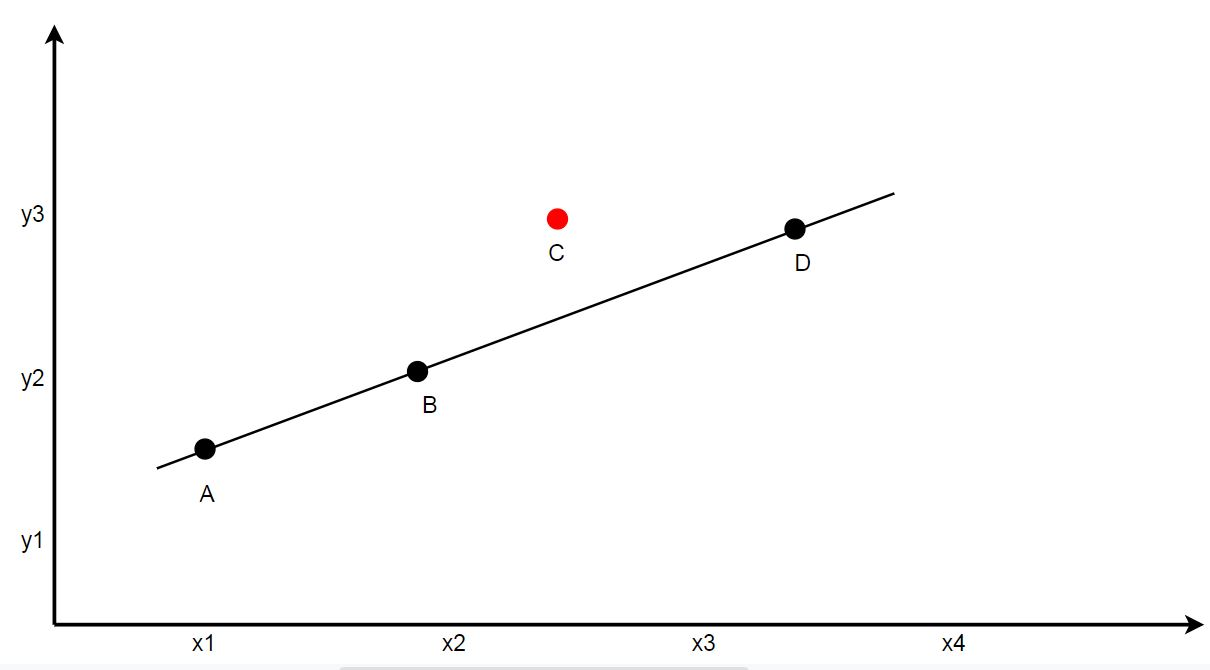
\includegraphics[width=\linewidth]{point.JPG}
  \caption{C is showing point anomaly.}
  \label{fig:point}
\end{figure}

\begin{figure}[bth]
  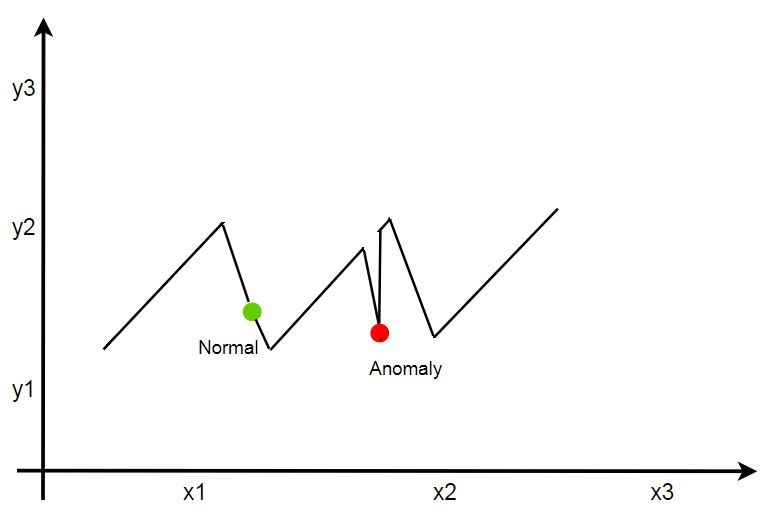
\includegraphics[width=\linewidth]{contextual.JPG}
  \caption{Contextual anomaly.}
  \label{fig:point}
\end{figure}

\begin{figure}[h]
  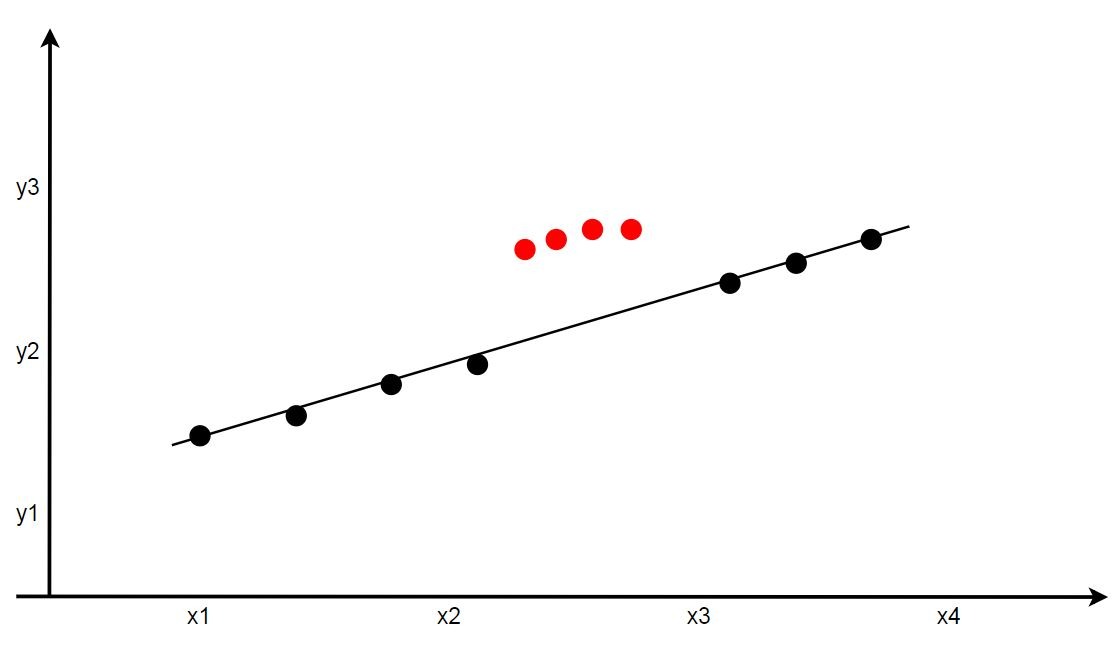
\includegraphics[width=\linewidth]{collective.JPG}
  \caption{4 red points are collectively showing anomaly.}
  \label{fig:point}
\end{figure}

There are different types of  attacks as follows:

\begin{itemize}
    \item \textbf{DoS attack}: DoS or Denial of Service represents the type of attack where the attacker makes a machine or resource unavailable to the legit users by blocking it intentionally through flooding. This attack keeps the memory resources of the server full so that legitimate user requests can not get through. Therefore, the user requests are denied.
    \item \textbf{Probe attack}: This type of attack is used to gather information about a targeted network or host and, more formally, for reconnaissance purposes ~\cite{ahmed2016survey}. This is used to know about the number \& type of machines connected in the network \& to know about installed softwares in the host machine. This is the step before an actual attack.
    \item \textbf{User to Root (U2R)}: When attacker wants to gain illegal access to an administrative account, U2R attack is used. Attacker can use social engineering approach or password sniffing \& being successful on those efforts, can access a normal user account. After gaining access in normal account \& exploiting vulnerabilities, attacker can gain the privilege of a super user.
    \item \textbf{Remote to User (R2U)}: It is launched when an attacker wants to gain local access as a user of a targeted machine to have the privilege of sending packets over its network (also known as R2L) ~\cite{ahmed2016survey}. Normally the attacker uses a trial and error method to guess the password. In some sophisticated attacks, attacker installs a sniffing tool to capture the password before going through the system.
\end{itemize}

Ahmed et al. ~\cite{ahmed2016survey} mapped the point anomaly with the U2R \& the R2U attacks. These type of attacks are condition specific and are hard to launch compared to other attacks. They mapped DoS attack to collective anomaly ~\cite{ahmed2014network} and Probe attack to contextual anomaly. DoS attack is specified by the collective attack of same nature. That is why it is mapped to collective anomaly as numerous connection requests are sent to deliver this attack. As probing is done on specific intention of gathering information, it is mapped with contextual anomaly.

\begin{figure}[b]
  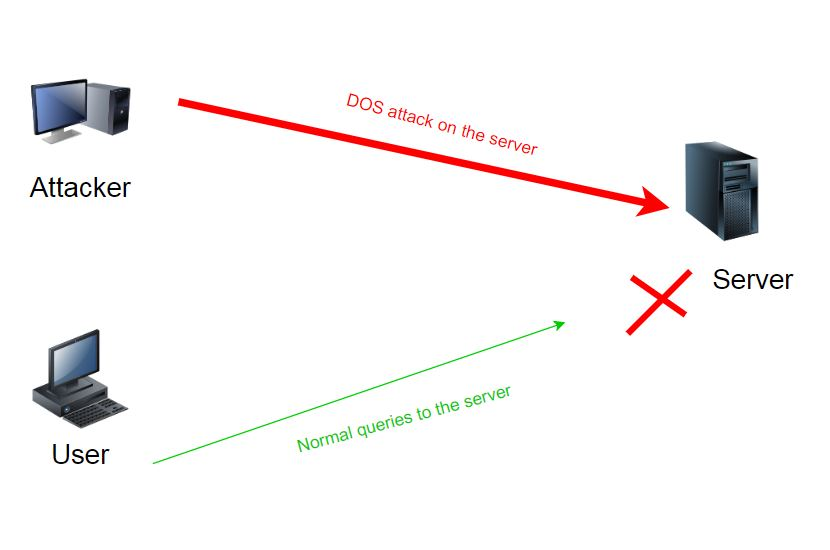
\includegraphics[width=\linewidth]{DOS2.JPG}
  \caption{DOS attack.}
  \label{fig:DOS}
\end{figure}



\section{Relevant works \label{relevant}}
Eskin et al. ~\cite{eskin2002geometric} used the concept of the unsupervised SVM to detect anomalous events. 
% 
Hu et al.~\cite{hu2003robust} presented an anomaly detection method using the Robust SVM (RSVM).  Yin et al.~\cite{yin2017deep} used deep learning on NSL-KDD (2009) dataset.

Zhu et al.~\cite{zhu2018deep} used the attention-base Multi-Flow LSTM on CICIDS2017 dataset and achieved about 10\% improvement in accuracy and recall on the multi-classification problems..

 UNSW-NB15 is one of the benchmark datasets in anomaly detection. It was introduced by moustafa et al.~\cite{moustafa2015unsw}. The state of the art work on this dataset was done in ~\cite{moustafa2018anomaly}, where the authors  used a beta mixture model. Mixture models are probabilistic models for representing sub-populations within an overall population. 

However, in recent times of machine learning and deep learning models have outperformed previous state of arts models on many occasions \cite{8264962}, \cite{7777224},~\cite{zhu2018deep}.

The state of the art work \cite{moustafa2018anomaly} on UNSW-NB15 dataset used Beta Mixture Model (a statistical and probabilistic model) to perform anomaly detection. Other models studied were also statistical ones. Machine learning and deep learning techniques have not yet been extensively applied to this dataset. Although the state of the art work on UNSW-NB15 has a low false alarm rate, its detection rate and accuracy can be further improved.
    
Therefore,  in this paper, we have proposed an ensemble of machine learning and deep learning models, trained and tested on  the UNSW-NB15 dataset~\cite{moustafa2015unsw}. 



%-------------------------------------------------------------

\section{Proposed Methodologies \label{methodology}}
In this section, we provide description about the dataset used, how it was pre-processed for using in model training. Then we explain the experimentation methods, how we trained and tested the models. Lastly, we provide the performance metrics used to evaluate and compare the results. 

%--- **** Importance of the DATASET  ******
\subsection{Dataset Description}
For our study, we have used a popular benchmark dataset in NIDS  research community, namely UNSW-NB15~\cite{moustafa2015unsw}  which is a hybrid of the real normal and modern synthesized attack of network data. It contains nine major families of attack types, such as  fuzzers, analysis, backdoor, DoS, exploit, generic, reconnaissance, shellcode and worm. In \cite{moustafa2015unsw}, \cite{moustafa2016evaluation} the authors have discussed the benefits of this dataset compared to other benchmark datasets, such as KDD98, KDDCUP99 and NSLKDD.


Following the previous works, we have used the part of this dataset provided in \cite{moustafa2016evaluation} which is separated in train and test set. Since, the dataset is labelled, we have implemented machine learning algorithms for network anomaly detection in supervised learning. There are a total of 44 features. We have transformed all anomaly classes into a single class for binary classification. Table ~\ref{unsw_nb15_des} shows the UNSW-NB15 dataset description.


\begin{table}[ht]
% this increases the fontsize used in table
\normalsize

\centering
\caption{UNSW-NB15 dataset description}
\label{unsw_nb15_des}
% increases cell padding
\renewcommand{\arraystretch}{1.2}

\begin{tabular}{|C{3cm}|C{1.6cm}|C{1.6cm}|}
\hline
\textbf{Attack type} & \textbf{Train} & \textbf{Test} \\ \hline
Normal & 37000 & 56000  \\ 
\hline
Anomaly & 45322 & 119341 \\ 
\hline
\textbf{Total} & \textbf{82322}  & \textbf{175341} \\ \hline
\end{tabular}
\end{table}


\subsection{Pre-processing}
We have performed the preprocessing on the data set using the following three steps: droppoing unnnecessary columns, numericalization and scaling. Details are descibed as follows.

\subsubsection{Dropping unnecessary columns}
We have dropped ID columns from both train and test dataset as those can not be learned as features. Also, source and destination IP addresses and port numbers were excluded from the feature set.

\subsubsection{Numericalization}
As machine learning requires input data to be in numeric format, we have converted each categorical column into numeric by creating binary columns for each of their attributes. However, test set had 6 nominal values which never appeared in the train dataset. As they were absent in train data, model had no way of learning from them. So we have dropped the binary columns for these labels. Finally, we had 188 features in our train data set.

\subsubsection{Scaling}
We have applied standard scaling using StandardScaler from sklearn's preprocessing library. This scaler calculates the mean and standard deviation of training  samples and converts them using the following equation: 
\begin{equation}
    x = \frac{x-\mu}{\sigma}
\end{equation}

where, $\mu$ is the mean value and $\sigma$ is the standard deviation. 

\subsection{Methodology}
For our machine learning models, we have used sklearn library of python and  for neural network, we used Keras  \footnote{https://keras.io/}, a python deep learning library developed by Google. We used kaggle \footnote{http://kaggle.com} kernels with GPU enabled to run our models. 

As the dataset comes with separate train and test set, we have trained the models on train data and varied different parameters to show the impact on the test data. For each model, we have presented the baseline parameters, parameters used in hyper-tuning and how varying parameters impacted the classification results.
Then finally we ensemble the predictions of the best performing models and give the final performance result in Section \ref{ensemble}. Models used in ensemble are RandomForest, GradientBoosting, XGB, LightGBM, Neural Network(dense layer based).


\subsection{Evaluation metrics}
Here, we discuss all The performance metrics used to compare the performance of our approach with previous works.
\begin{itemize}
    \item \textbf{True Positives (TP)} : The cases in which we predicted YES and the actual output was also YES.
    \item \textbf{True Negatives (TN} : The cases in which we predicted NO and the actual output was NO.
    \item \textbf{False Positives (FP)} : The cases in which we predicted YES and the actual output was NO.
    \item \textbf{False Negatives (FN)} : The cases in which we predicted NO and the actual output was YES.
\end{itemize}

\subsubsection{Accuracy}
It is the ratio of number of correct predictions to the total number of input samples
\begin{equation}
    Accuracy = \frac{TP+TN}{TP+TN+FP+FN}
\end{equation}

\subsubsection{Precision}
It is the number of correct positive results divided by the number of positive results predicted by the classifier.
\begin{equation}
    precision = \frac{TP}{TP+FP}
\end{equation}

\subsubsection{Recall or DR(Detection Rate)}
It is the number of correct positive results divided by the number of all relevant samples (all samples that should have been identified as positive)
\begin{equation}
    recall = \frac{TP}{TP+FN}
\end{equation}

\subsubsection{FPR}
The false positive rate (FPR) is the proportion of incorrectly identified observations, that is 
\begin{equation}
    FPR = \frac{FP}{FP+TN}
\end{equation}

\subsubsection{F1-score}
F1-score is the harmonic Mean between precision and recall.
\begin{equation}
    f1\_score = 2 * \frac{1}{\frac{1}{precision}+ \frac{1}{recall}}
\end{equation}


\section{Experiment and Results \label{results}}
In this section, we describe experimentation methods and results of various machine learning based models on unsw-nb15 dataset. In each part, we have described the hypertuning part of a model and the best possible results from it. The best results are marked using * in each table.\\

\subsection{RandomForestClassifier}
We have used RandomForestClassifier from sklearn.ensemble. The baseline parameters are listed in Table~\ref{rf_base_parameters}. We set prediction threshold at 0.4 for this model. From Table~\ref{rf_table}, we can see that changing max depth did not have much effect on the model performance except reducing it a bit. However, when we increase the number of estimators beyond 100,  the accuracy decreases. This is because the model then overfits on train data. 


%Table \ref{rf_table} contains the hyper-tuning results. Base parameters of the classifier are given below.

\begin{table}[H]
% this increases the fontsize used in table
\normalsize

\centering
\caption{RandomForest baseline parameters}
\label{rf_base_parameters}
% increases cell padding
\renewcommand{\arraystretch}{1.2}

\begin{tabular}{|C{2.6cm}|C{1cm}|C{2.7cm}|C{1cm}|}
\hline
\textbf{Parameter} & \textbf{Value} & \textbf{Parameter} & \textbf{Value} \\ \hline
% criterion & ’gini’ &  min\_samples\_split  & 2   \\ \hline
min\_samples\_leaf & 1 & class\_weight & None  \\ \hline
max\_features & ’auto’& max\_leaf\_nodes & None  \\ \hline
%min\_impurity\_decrease & 0.0 & min\_impurity\_split & None  \\ \hline
% warm\_start & False & oob\_score & False  \\ \hline
 bootstrap & True & random\_state & 0  \\ \hline
%min\_weight\_fraction\_leaf & 0.0 & &  \\ \hline
\end{tabular}
\end{table}

Also, decreasing the estimators less than 100 has negative impact on the performance. The best model was achieved with 100 estimators and max depth at 50 (see Table~\ref{rf_table}).

\begin{table}[H]
% this increases the fontsize used in table
\normalsize

\centering
\caption{RandomForest classifier results}
\label{rf_table}
% increases cell padding
\renewcommand{\arraystretch}{1.2}

\begin{tabular}{|C{2cm}|C{1.2cm}|C{1.6cm}|C{1.6cm}|}
\hline
\textbf{n-estimators} & \textbf{depth} & \textbf{accuracy} & \textbf{f1-score} \\ \hline
50 & 50 & 93.24 & 95.22 \\ \hline
50 & 150 & 93.33 & 95.27 \\ \hline
100 & 50 & 93.39* & 95.31* \\ \hline
100 & 150 & 93.33 & 95.27 \\ \hline
200 & 50 & 93.36 & 95.30 \\ \hline
200 & 150 & 93.34 & 95.29\\ \hline
500 & 50 & 93.03 & 95.31 \\ \hline
500 & 150 & 93.01 & 95.29 \\ \hline
\multicolumn{4}{l}{$*$ best parameters}
\end{tabular}
\end{table}

\subsection{GradientBoosting}
We have used GradientBoostingClassifier from sklearn.ensemble. We have varied n\_estimators and learning rate for this model. Each estimator has regression trees with maximum depth 3. We set prediction threshold at 0.5 for this model. The baseline parameters of this classifier are listed in Table~\ref{gtb_base_parameters}. From Table~\ref{gtb_table}, we find that with the increase  the number of estimators, the accuracy of the classifier is increased.
% The base parameters for this model are given in table \ref{gtb_base_parameters}.
\begin{table}[H]
% this increases the fontsize used in table
\normalsize

\centering
\caption{GradientBoosting baseline parameters}
\label{gtb_base_parameters}
% increases cell padding
\renewcommand{\arraystretch}{1.2}

\begin{tabular}{|C{2.7cm}|C{1cm}|C{2.6cm}|C{1cm}|}
\hline
\textbf{parameter} & \textbf{value} & \textbf{parameter} & \textbf{value} \\ \hline
learning\_rate & 0.1 & presort & ’auto’ \\ \hline
n\_estimators & 100 &  max\_depth & 3  \\ \hline
% subsample & 1.0 &  tol & 0.0001 \\ \hline
random\_state & 0 & max\_features & None \\ \hline
\end{tabular}
\end{table}
 We did not increase it further to prevent overfitting. Also, decreasing learning rate than 0.1 had negative impact on performance, because the model was learning too slow to converge.
\begin{table}[H]
\normalsize

\centering
\caption{GradientBoosting Classifier results}
\label{gtb_table}
\renewcommand{\arraystretch}{1.2}
\begin{tabular}{|C{2cm}|C{2cm}|C{1.5cm}|C{1.5cm}|}
\hline
\textbf{n-estimators} & \textbf{learning rate} & \textbf{accuracy} & \textbf{f1-score} \\ \hline
100 & 0.05 & 89.82 & 92.31 \\ \hline
100 & 0.1 & 92.09 & 94.12 \\ \hline
% 200 & 0.05 & 92.42 & 94.48 \\ \hline
% 200 & 0.1 & 92.30 & 94.36 \\ \hline
500 & 0.05 & 92.40 & 94.49 \\ \hline
500 & 0.1 & 92.61* & 94.67* \\ \hline
\multicolumn{4}{l}{$*$ best parameters}
\end{tabular}
\end{table}

\subsection{LightGBM}
LightGBM is a gradient boosting framework from Microsoft that uses tree based learning algorithms. 
%The baseline parameters are given in table \ref{lgb_table}.

\begin{table}[H]
% this increases the fontsize used in table
\normalsize

\centering
\caption{LightGBM baseline parameters}
\label{lgb_base_parameters}
% increases cell padding
\renewcommand{\arraystretch}{1.2}

\begin{tabular}{|C{3.1cm}|C{1cm}|C{2.5cm}|C{0.8cm}|}
\hline
\textbf{parameter} & \textbf{value} & \textbf{parameter} & \textbf{value} \\ \hline
bagging\_frequency & 5 & base\_score & 0.9 \\ \hline
early\_stopping\_round & 100 & boost & gbdt \\ \hline
num\_boost\_round & 2000  & max\_bin & 255\\ \hline
objective & binary & num\_leaves & 31 \\ \hline
\end{tabular}
\end{table}
The baseline parameters for the LightGBM model are listed in Table~\ref{lgb_base_parameters}. We have varied four parameters of this model: learning rate, max-depth, bagging fraction, feature fraction. We set prediction threshold at 0.4 for this model. From Table~\ref{lgb_table} we find that when the learning rate is decreased, the performance (accuracy) of the model also decreased. This is because it fails to convergence with a slower learning rate.
%
We found setting constraint on depth gives improved results. Among them, best results was found at depth 10. Also, adding fraction less than 1.0 improved classifier performance, this fraction means what fraction of the dataset and features would be used for training in the next iteration. 

\begin{table}[H]
\normalsize

\centering
\caption{LightGBM results}
\label{lgb_table}
\renewcommand{\arraystretch}{1.2}
\begin{tabular}{|C{1.4cm}|C{1.2cm}|C{1.6cm}|C{1.2cm}|C{1.2cm}|}
\hline
\textbf{learning rate} & \textbf{max depth} & \textbf{bagging and feature fraction} & \textbf{accuracy} & \textbf{f1-score} \\ \hline
0.1 & 10 & 0.5 & 92.69 & 94.71 \\ \hline
0.1 & 10 & 1 & 92.75* & 94.78* \\ \hline
0.1 & 15 & 0.5 & 92.63 & 94.69 \\ \hline
0.1 & 15 & 1 & 92.59 & 94.67 \\ \hline
0.01 & 10 & 0.5 & 92.75 & 94.69 \\ \hline
0.01 & 10 & 1 & 92.55 & 94.59 \\ \hline
0.01 & 15 & 0.5 & 92.84 & 94.76 \\ \hline
0.01 & 15 & 1 & 92.59 & 94.62 \\ \hline
\multicolumn{5}{l}{$*$ best parameters}
\end{tabular}
\end{table}

\subsection{XGBClassifier}
XGBoost is an optimized distributed gradient boosting library. We have worked on the XGBClassifier from XGBoost. We have replaced the base score with 0.9, as it improved the performance. Prediction threshold was set to 0.2. From Table~\ref{xgb_table}, we can see that performance decreases randomly with the increase of number of estimators. However, the result improved for higher learning rate. But increasing learning rate too much can made the model fail to converge. 



\begin{table}[H]
\normalsize
\centering
\caption{XGB Classifier results}
\label{xgb_table}

\renewcommand{\arraystretch}{1.2}
\begin{tabular}{|C{2cm}|C{2cm}|C{1.5cm}|C{1.5cm}|}
\hline
\textbf{n-estimators} & \textbf{learning rate} & \textbf{accuracy} & \textbf{f1-score} \\ \hline
100 & 0.1 & 91.45 & 93.71 \\ \hline
100 & 0.5 & 92.13* & 94.34* \\ \hline
500 & 0.1 & 91.94 & 94.23 \\ \hline
500 & 0.5 & 90.42 & 93.3 \\ \hline
\multicolumn{4}{l}{$*$ best parameters}
\end{tabular}
\end{table}

\subsection{Artificial Neural Network}
% An ANN is based on a collection of connected units or nodes called artificial neurons, which loosely model the neurons in a biological brain. Each connection, like the synapses in a biological brain, can transmit a signal from one artificial neuron to another. An artificial neuron that receives a signal can process it and then signal additional artificial neurons connected to it.\\
We used Keras framework for implementing neural network. We tried different combination of layers, units of dense and dropout layer. Dense layer is a densely connected neural network layer, which connects every input to every cell unit. Dropout layer randomly sets a fraction of input units to 0, reducing overfit. 

Our number of epochs was 10 and we took the best model based on validation accuracy. From our results (shown in Table~\ref{nn_table}), we can see that increasing input layer size increases model performance, because it helps to learn more from the input data. However, using more layers caused the model to overfit. Also adding dropout layer did not solve the issue. So, the best model was a neural network with 512 dense input units, then 32 dense input units, following the final output unit. All dense layers except the last one used activation method 'relu'. The last layer had activation method 'sigmoid'.


\begin{table}[H]
\normalsize

\centering
\caption{ANN results}
\label{nn_table}
\renewcommand{\arraystretch}{1.2}
\begin{tabular}{|C{5.6cm}|C{1cm}|C{1cm}|}
\hline
\textbf{Model architecture} & \textbf{accuracy} & \textbf{f1-score} \\ \hline
dense(256)dense(32)dense(1) & 91.97 &  94.01 \\ \hline
dense(256)drop(.2)dense(32)dense(1) & 91.84 & 93.86 \\ \hline
dense(256)dense(64)dense(32)dense(1)  & 91.82 & 93.84 \\ \hline
dense(512)dense(32)dense(1)  & 92.05* & 94.06* \\ \hline
\multicolumn{3}{l}{$*$ best architecture}
\end{tabular}
\end{table}


\subsection{Ensemble \label{ensemble}}
Ensemble method is a machine learning technique that combines several base models in order to produce one optimal predictive model. In this part, we have taken our best performing models and used their predictions to give the final output. For each model, the best performing one is marked by * sign.

% The list of the models with their hyper-tuned parameters is available in table \ref{ensemble_table}.
% \begin{table*}[h]
% \normalsize
% \centering
% \caption{Models used in ensemble}
% \label{ensemble_table}
% \renewcommand{\arraystretch}{1.2}
% \begin{tabular}{|C{3cm}|C{4cm}|C{3cm}|C{2.5cm}|}
% \hline
% \textbf{Model} & \multicolumn{3}{c}{\textbf{parameters}}  \\ \hline
% RandomForest & n\_estimators=100 & max\_depth=50 & random\_state=0\\ \hline
% GradientBoosting & n\_estimators=500 & learning\_rate=0.1 & random\_state=0 \\ \hline
%  XGBClassifier & n\_estimators=1000 & learning\_rate=0.1 & base\_score=0.9 \\ \hline
% LigtGBM.& bagging\_fraction=0.8 & learning\_rate=0.01 & max\_depth=15 \\ \hline
% Neural Network & dense(512) & dense(32) & dense(1) \\ \hline
% \end{tabular}
% \end{table*}

There are several ways ensemble can be used. We took a simple approach called majority voting. It works by taking prediction from everyone and giving the output in favour of the class for which most of the models gave same output. After applying voting on the predictions of all models on test data our final result reached 93.69\% accuracy, 93.24\% precision, 97.82\% recall and 95.48\% f1-score on the test dataset. 

\section{Comparison with state of the art \label{comparison}}
Our final model achieves 93.69\% accuracy, 93.24\% precision, 97.82\% recall and 95.48\% f1-score on the separate test dataset. Our ROC-AUC score is 98.45\% which is also very high.\\

Compared to previous works, our model outperforms the state of the art model by Moustafa et al.~\cite{moustafa2018anomaly} as we can see from table \ref{comparison_table}. However, our FPR is 15.11\%, which is higher than theirs, so our false alarm rate is higher than their work.

\begin{table}[H]
\normalsize
\centering
\caption{Comparison with state of the art}
\label{comparison_table}
\renewcommand{\arraystretch}{1.2}
\begin{tabular}{|C{2.5cm}|C{3cm}|C{2cm}|}
\hline
Metrics & Moustafa \textit{et al.}\cite{moustafa2018anomaly} & Our Model\\ \hline
DR(\%) & 92.70 & 97.82* \\ \hline
Accuracy(\%) & 93.40 & 93.69* \\ \hline
FPR(\%) & 5.90*  & 15.11 \\ \hline
\multicolumn{3}{l}{$*$ better result}
\end{tabular}
\end{table}


Our ensemble model has a greater detection rate which is possible as even if one model fails to detect an anomaly, there are other models which does not fail. Thus, this ensemble version detects more anomaly connections, thereby making our model better in terms of detection rate. 
%
However, as the ensemble model detects more connections as anomaly, it also makes more false alarms (meaning  normal connections as anomaly). That is why our false positive rate is higher than the previous work.

As our models ensembles several models, some of which takes much time to train. Hence, our model is slower to learn  compared to previous statistical based model. %Also as our false positive rate is higher, our model  tends to make more false alarms, which might be disturbing for the user.
Nevertheless, for sensitive connection and for better detection, our model is certainly  the better choice.

% \begin{figure}
% \centering
%   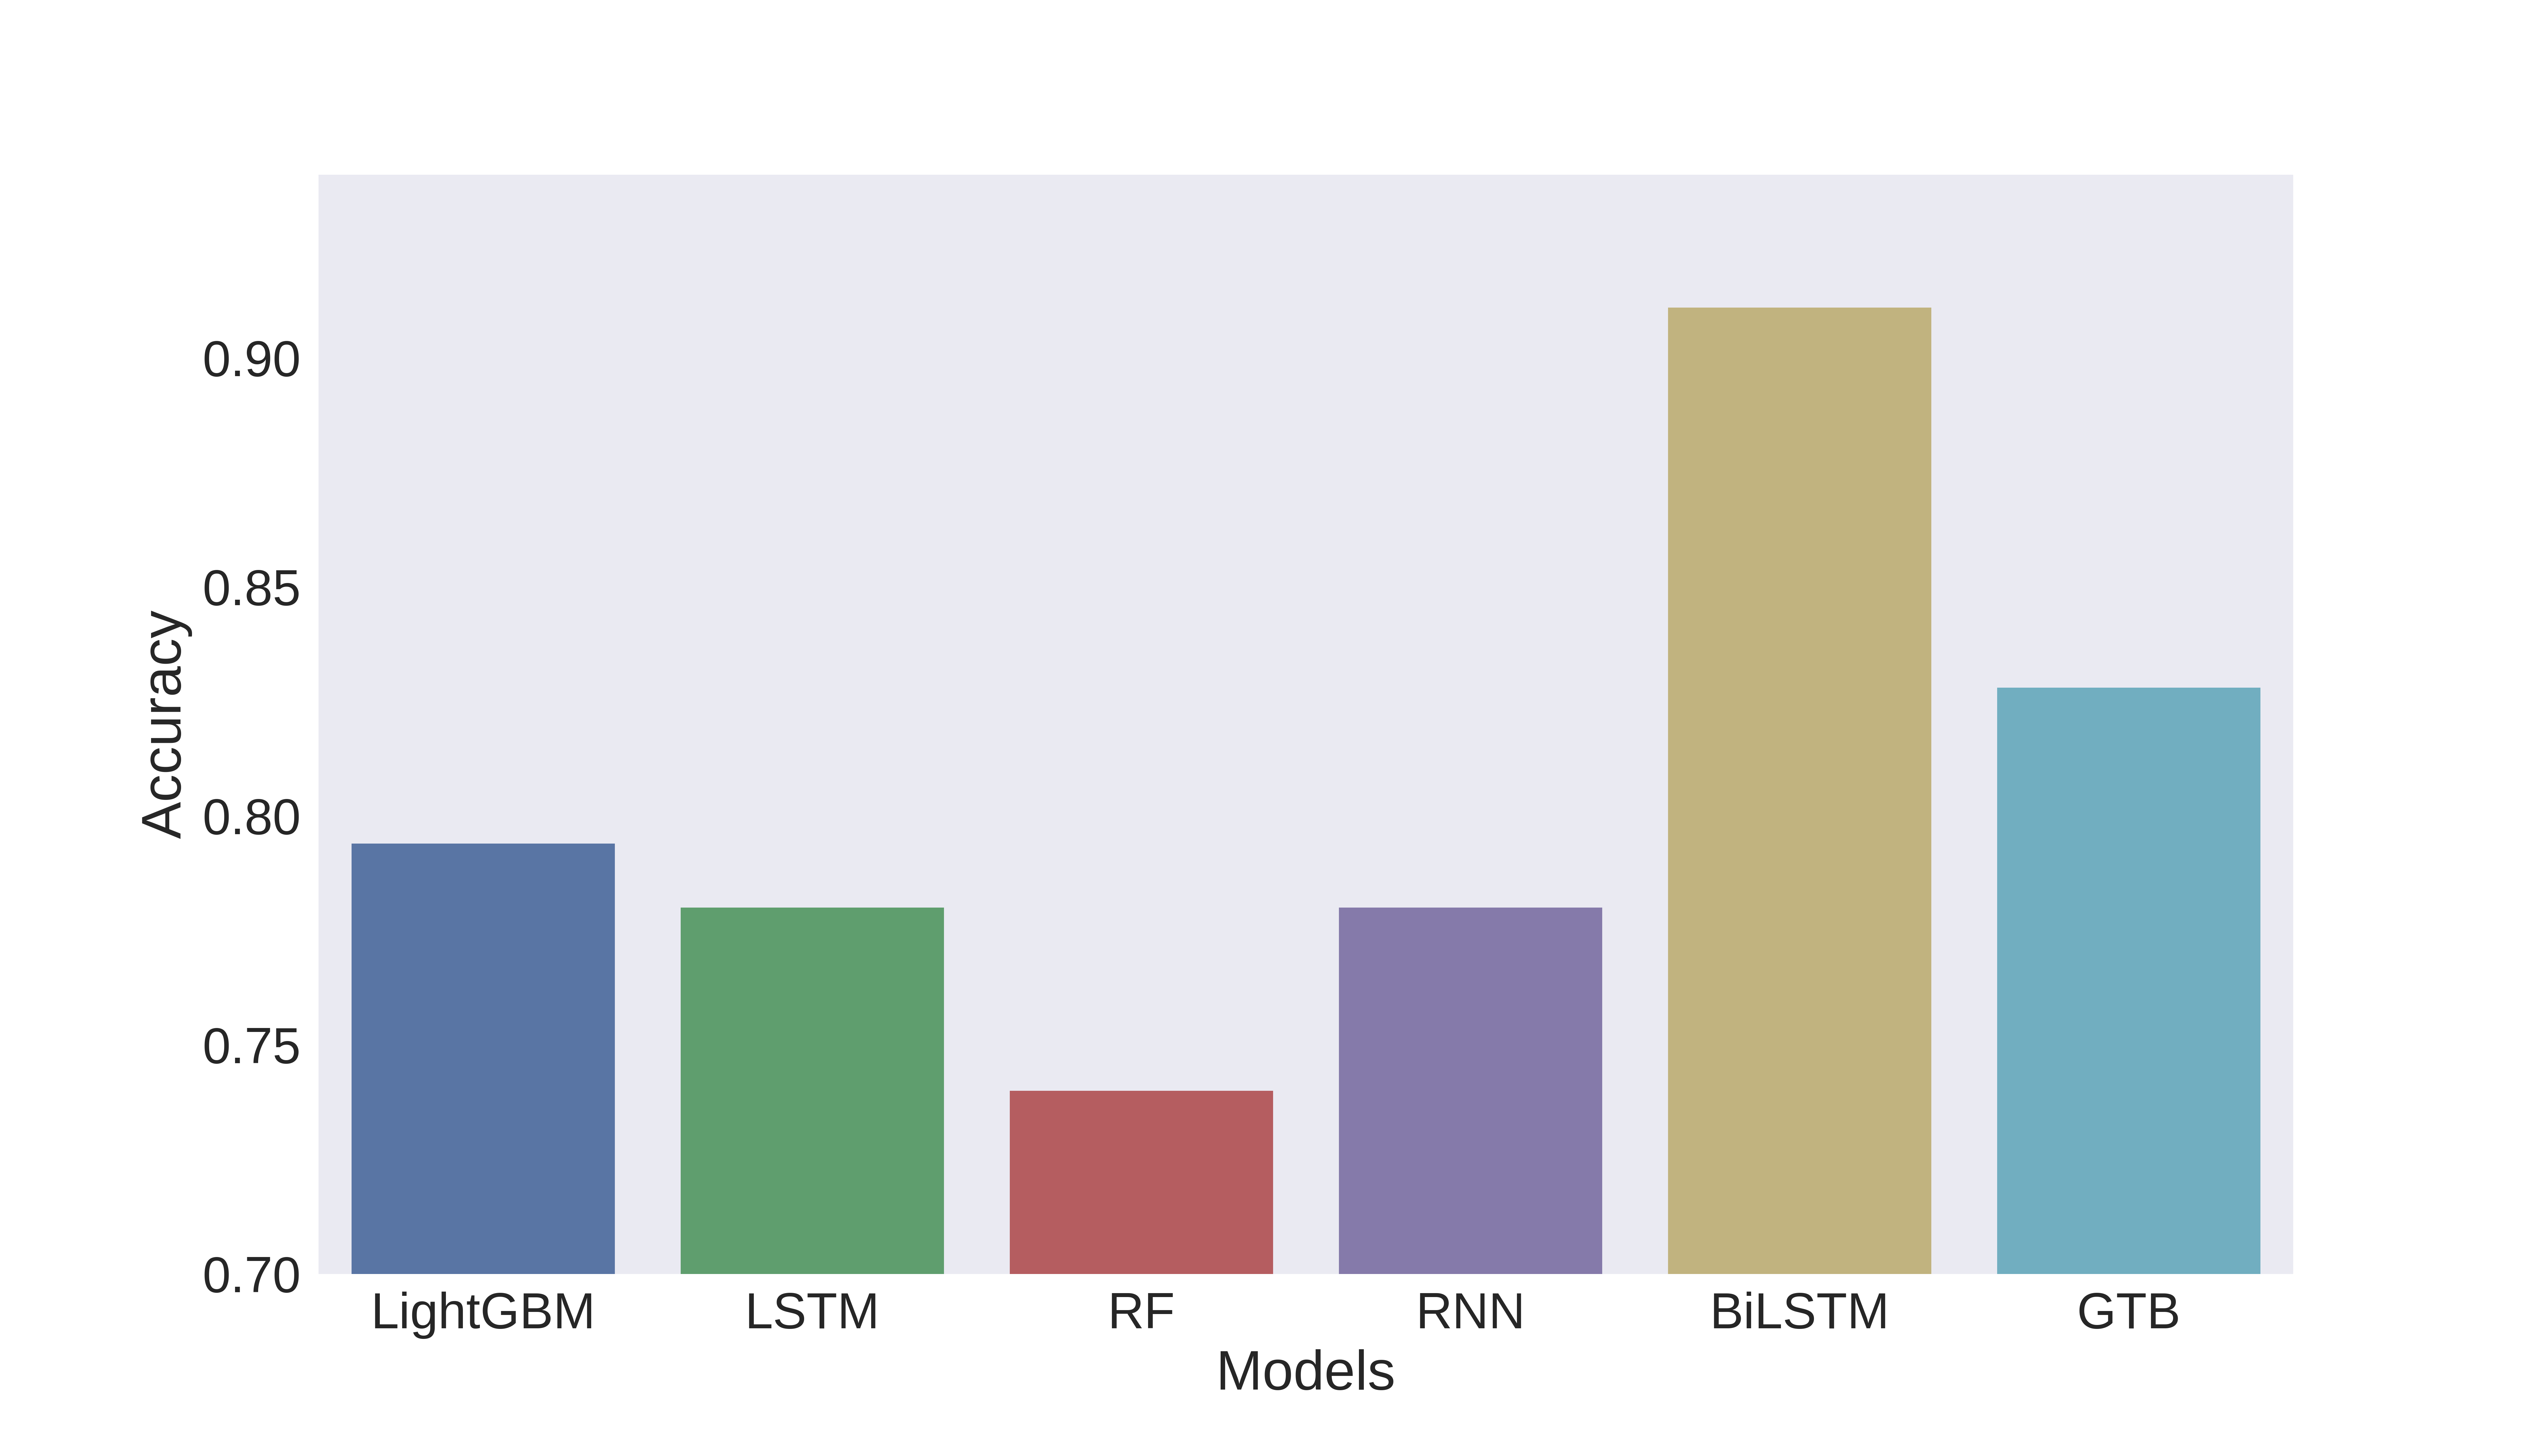
\includegraphics[scale=0.7,width=\linewidth]{UNSW_NB15_top_models_accuracy.png}
% \caption{Accuracy on UNSW-NB15}
% \end{figure}

% \begin{figure}
% \centering
%   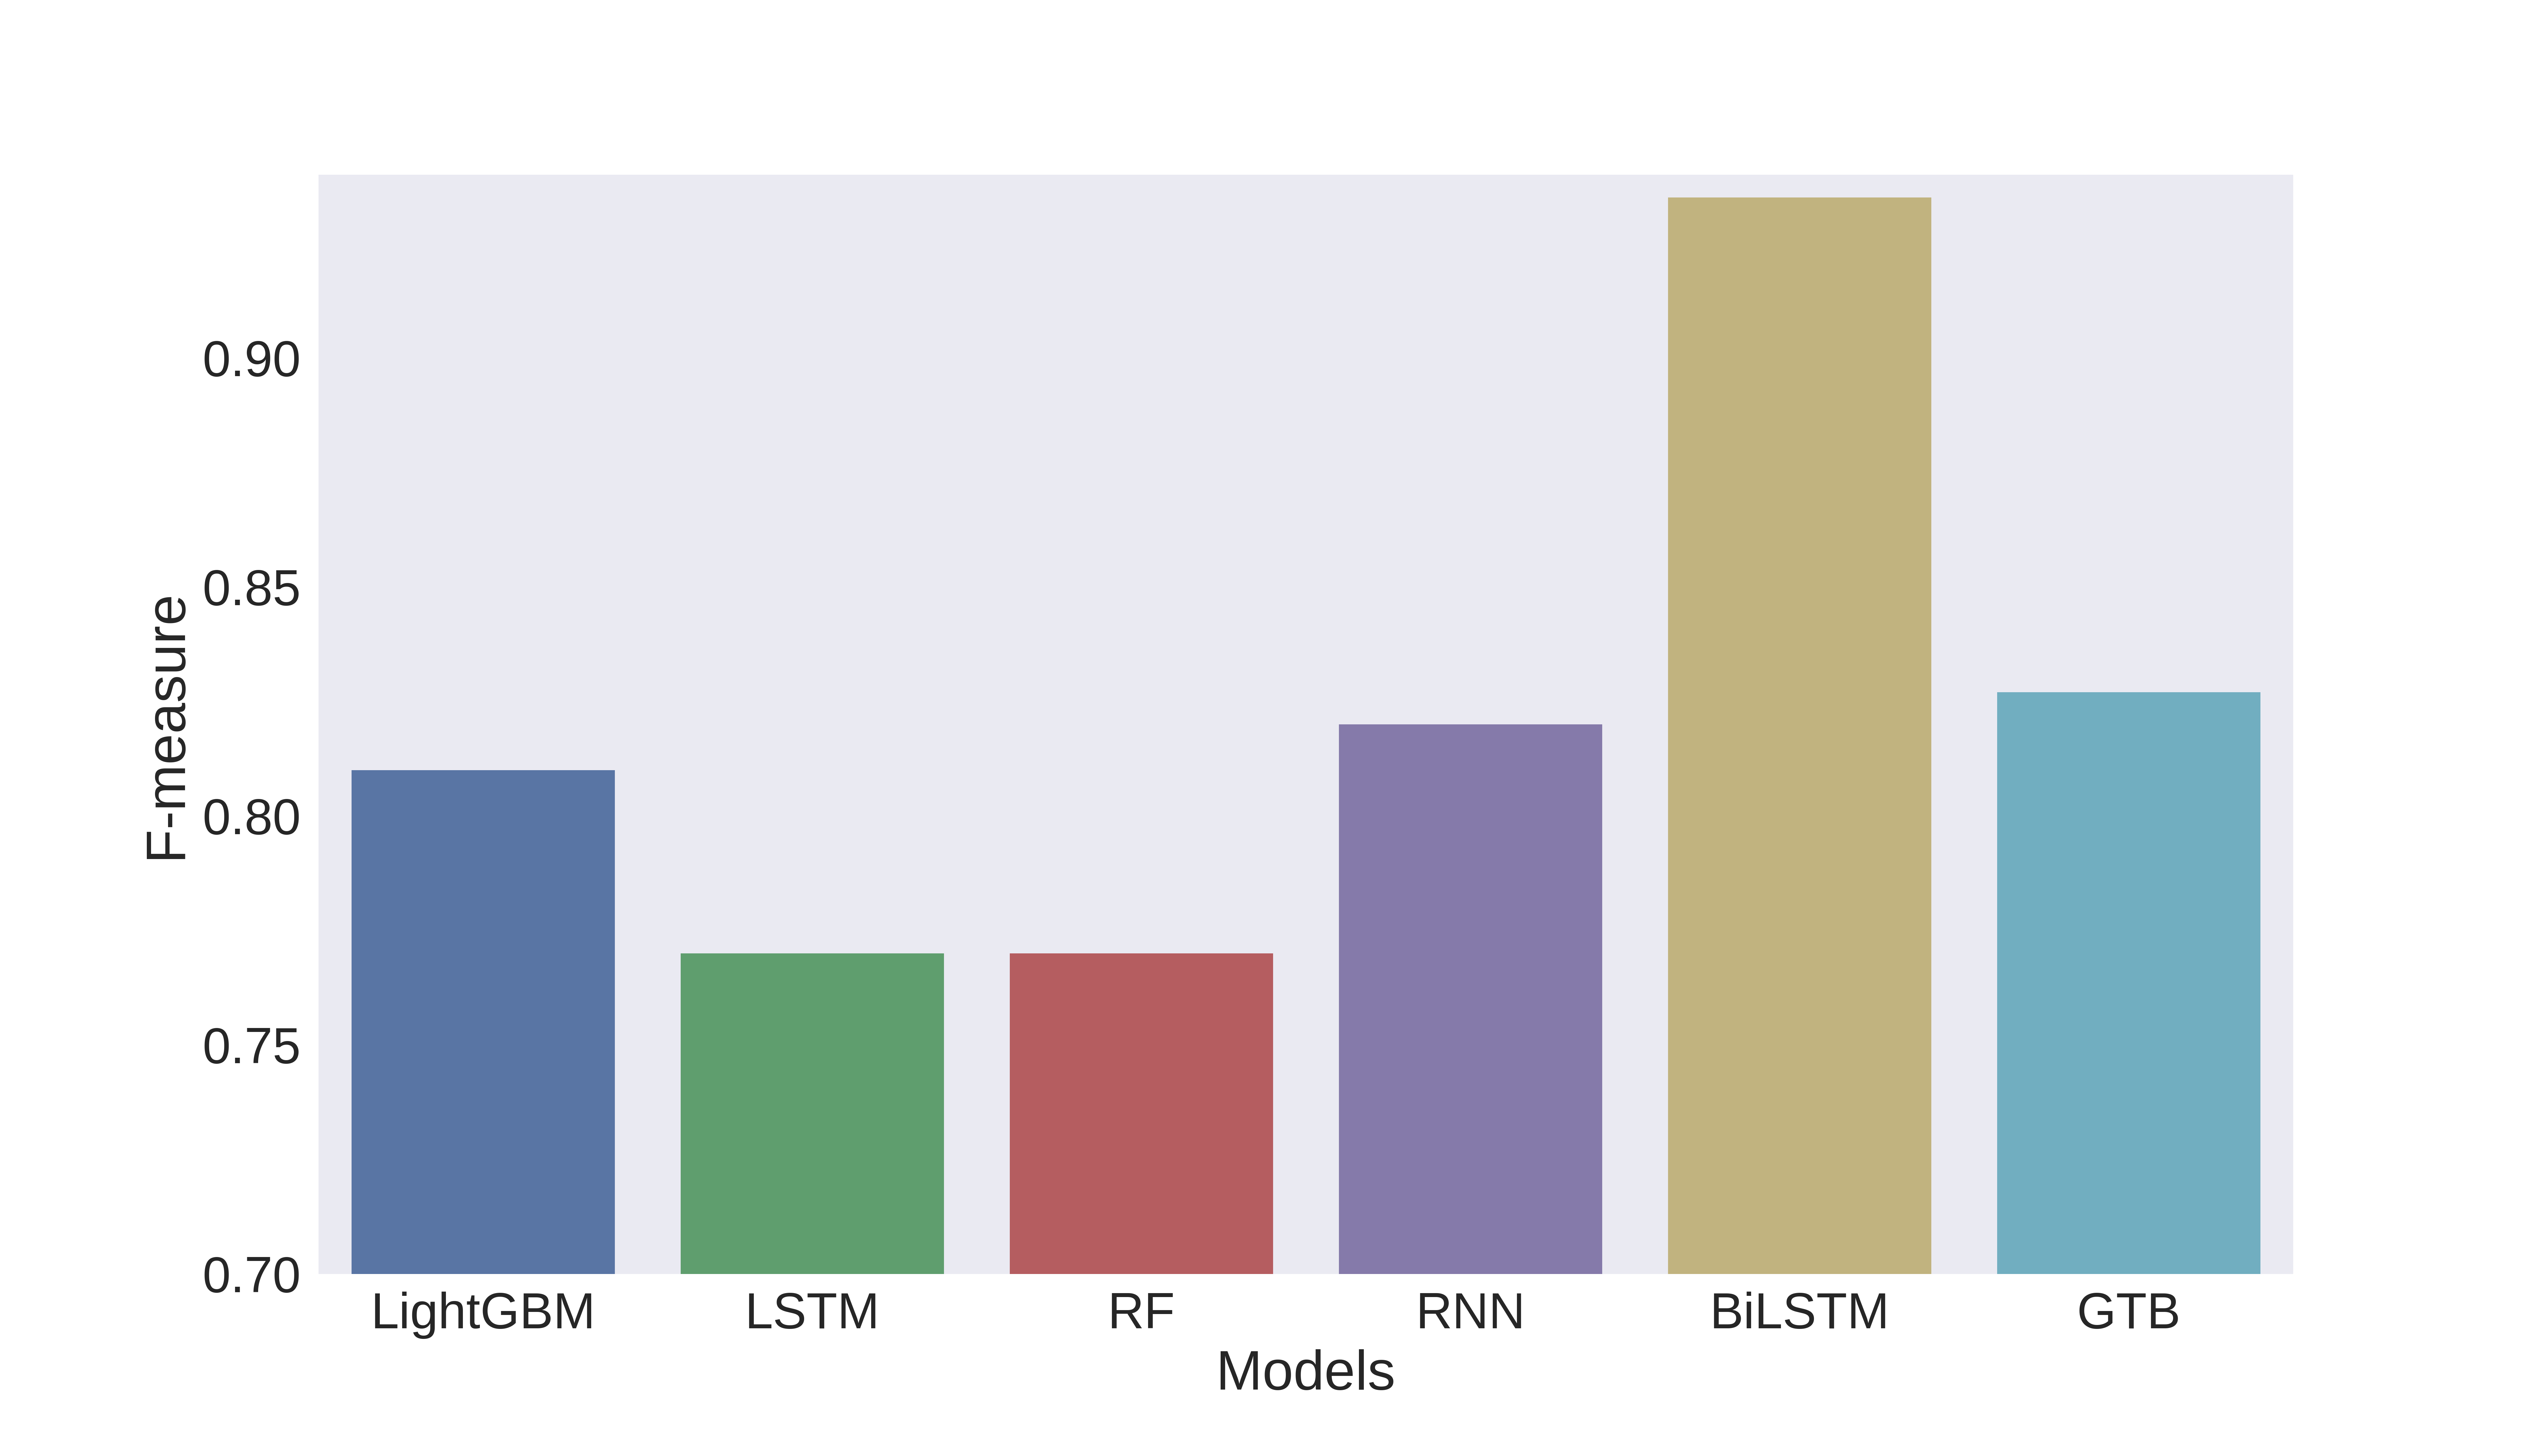
\includegraphics[scale=0.7,width=\linewidth]{UNSW_NB15_top_models_f_measure.png}

% \caption{F-measure on UNSW-NB15}
% \end{figure}





%---------------------------- Conclusion ----------------
%---------------------------- Conclusion ----------------
%---------------------------- Conclusion ----------------

\section{Conclusion}
\label{conclusion}

In this paper, we have  worked on a benchmark data set and proposed  an ensemble based machine learning for anomaly detection from the network traffic. Our ensemble of machine learning models, trained on UNSW-NB15 anomaly detection dataset, outperforms tne current  state of the art in terms of detection rate and accuracy. we have clearly shown how machine learning can be used on this dataset to surpass traditional probabilistic models. 


Our ensemble model has a greater detection rate which is because if one model fails to detect an anomaly, there are other models which does detect the anomaly. Thus, this ensemble version detects more anomalous connections, thereby making our model better in terms of detection rate. 


%However, our limitations are model complexity and higher false positive rate. Yet its an indication of success of this kind of technique to go beyond previous state of the art works, which is promising. 
%Also because of multiple models and complexity of machine learning algorithms this model would take longer to train and test. However, with the development of technological resources that should be less difficult for a system to deploy now.


\bibliography{bibliography} 

\end{document}


